% !TEX root =  ../ReplyLetterMain.tex
\clearpage
\section*{Response to 2nd Referee's Comments}
We would like to thank the Referee for his/her constructive comments, which have allowed us to considerably improve our paper. The main differences of the new version of the manuscript compared to the previous one can be found in Sections~5 and 6, Web Appendix A.2, C and D. In addition, changes regarding the specific comments have been made throughout the text.

You may find below our responses to the specific issues raised.

\begin{enumerate}
    \item [1,4.] \underline{Validity of the model for PSA.}

    We would like to thank the Referee for motivating us to check the model assumptions and fit. As the Referee noted, the equation for the longitudinal sub-model on page 4 of the original manuscript does not indicate that we used a log transform for PSA levels. This is however the general form of the equation for the longitudinal sub-model, and is only used to introduce the joint model (JM) notation. The actual equation, showing the log transformed PSA levels, baseline covariates and B-spline for the effect of time is Equation (\ref{eq : long_model_prias_ref2}) below (it is Equation \ref{eq : long_model_prias} in the revised manuscript). That is, it is not the case that the log transformation is used only in simulation study as noted by the referee, but also used for fitting the PRIAS data. 

    \begin{equation}
\label{eq : long_model_prias_ref2}
\begin{aligned}
\log_2 \mbox{PSA}(t) &= \beta_0 + \beta_1 (\mbox{Age}-70) + \beta_2 (\mbox{Age}-70)^2 + \sum_{k=1}^4 \beta_{k+2} B_k(t,\mathcal{K})\\ 
&+  b_{i0} + b_{i1} B_7(t, 0.1) + b_{i2} B_8(t, 0.1) +
\varepsilon_i(t),
\end{aligned}
\end{equation}

    Since concerns regarding assumption of normality on errors were also raised by the first Referee, we refitted our model with an assumption that the errors are t-distributed (df=3). The residual quantile-quantile plots for the model with normally distributed errors as well as the T-distributed (df=3) errors are shown in Figure \ref{fig : qqplot_norm_t3_ref2}. In addition, the fitted marginal $\log_2 \mbox{PSA}$ profiles, and subject specific fitted versus observed $\log_2 \mbox{PSA}$ profiles of 9 randomly selected patients, using the two different models are presented in Figure \ref{fig : marginal_fitted_psa_NormalVsT3_ref2} and Figure \ref{fig : subject_fittedVsObserved_psa_norm_t3_ref2}, respectively.

    \begin{figure}[!htb]
    \centerline{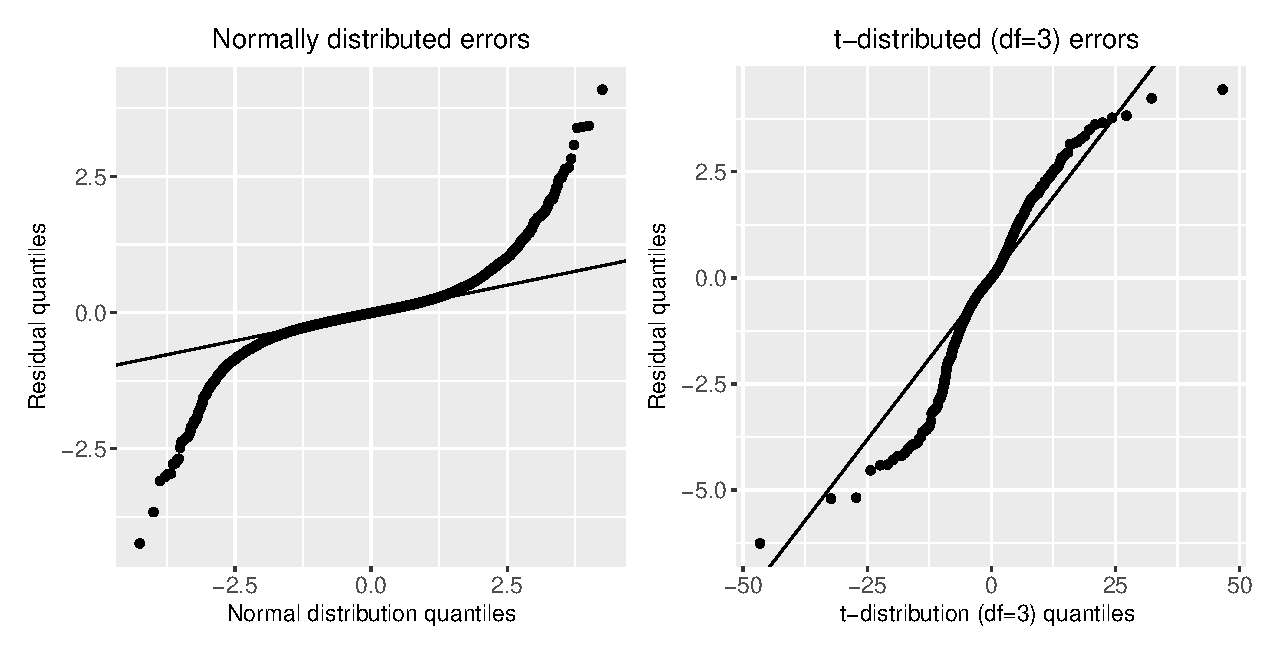
\includegraphics[width=\columnwidth]{images/model_fit/qqplot_norm_t3.eps}}
    \caption{Quantile-quantile plots of subject specific residuals obtained from joint models with assumption of normally distributed errors, and t-distributed (df=3) errors, fitted to the PRIAS data set.}
    \label{fig : qqplot_norm_t3_ref2}
    \end{figure}

\begin{figure}[!htb]
    \centerline{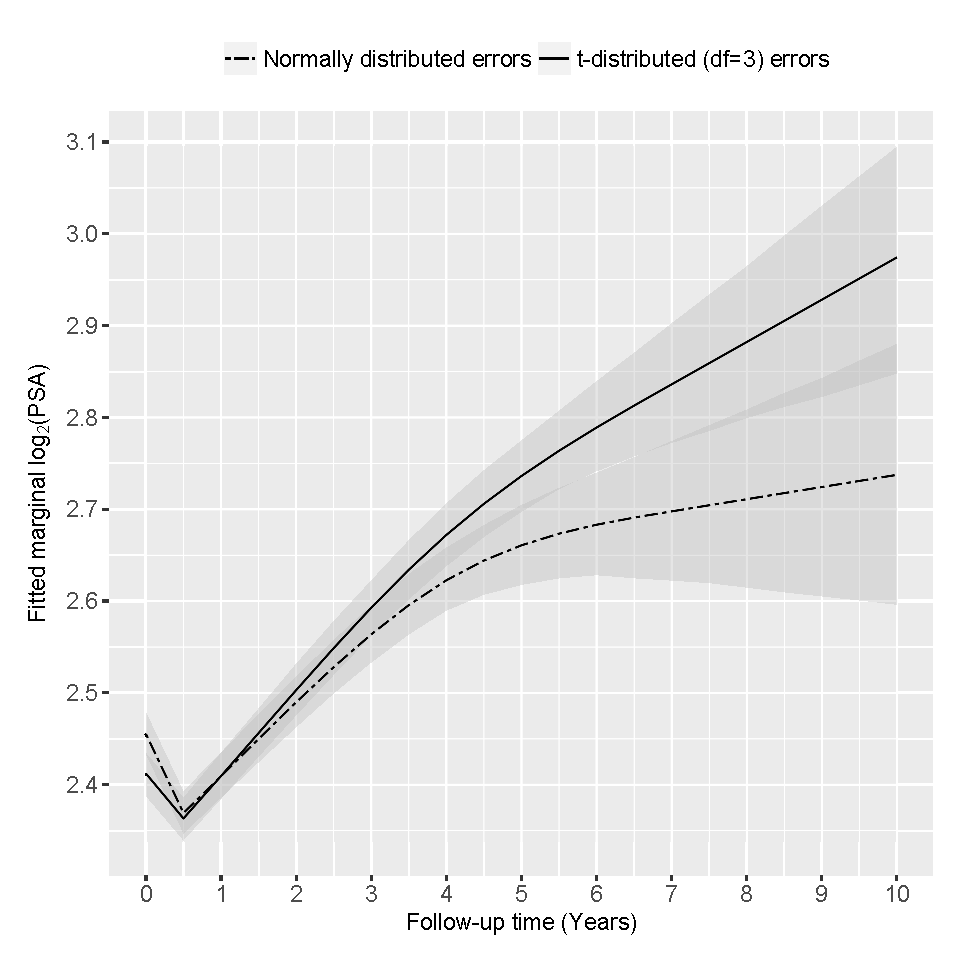
\includegraphics[width=0.75\columnwidth]{images/model_fit/marginal_fitted_psa_NormalVsT3.eps}}
    \caption{Fitted marginal 10 year $\log_2 \mbox{PSA}$ profile with 95\% credible interval (CI), for a hypothetical patient who was included in AS at the age of 70 years. Fits were obtained from joint models with assumption of normal distributed errors, and t-distributed (df=3) errors. The darker shaded region indicates the overlap in the two CI intervals, as well as demarcates the two sets of CIs.}
    \label{fig : marginal_fitted_psa_NormalVsT3_ref2}
    \end{figure}        
    
    \begin{figure}[!htb]
    \centerline{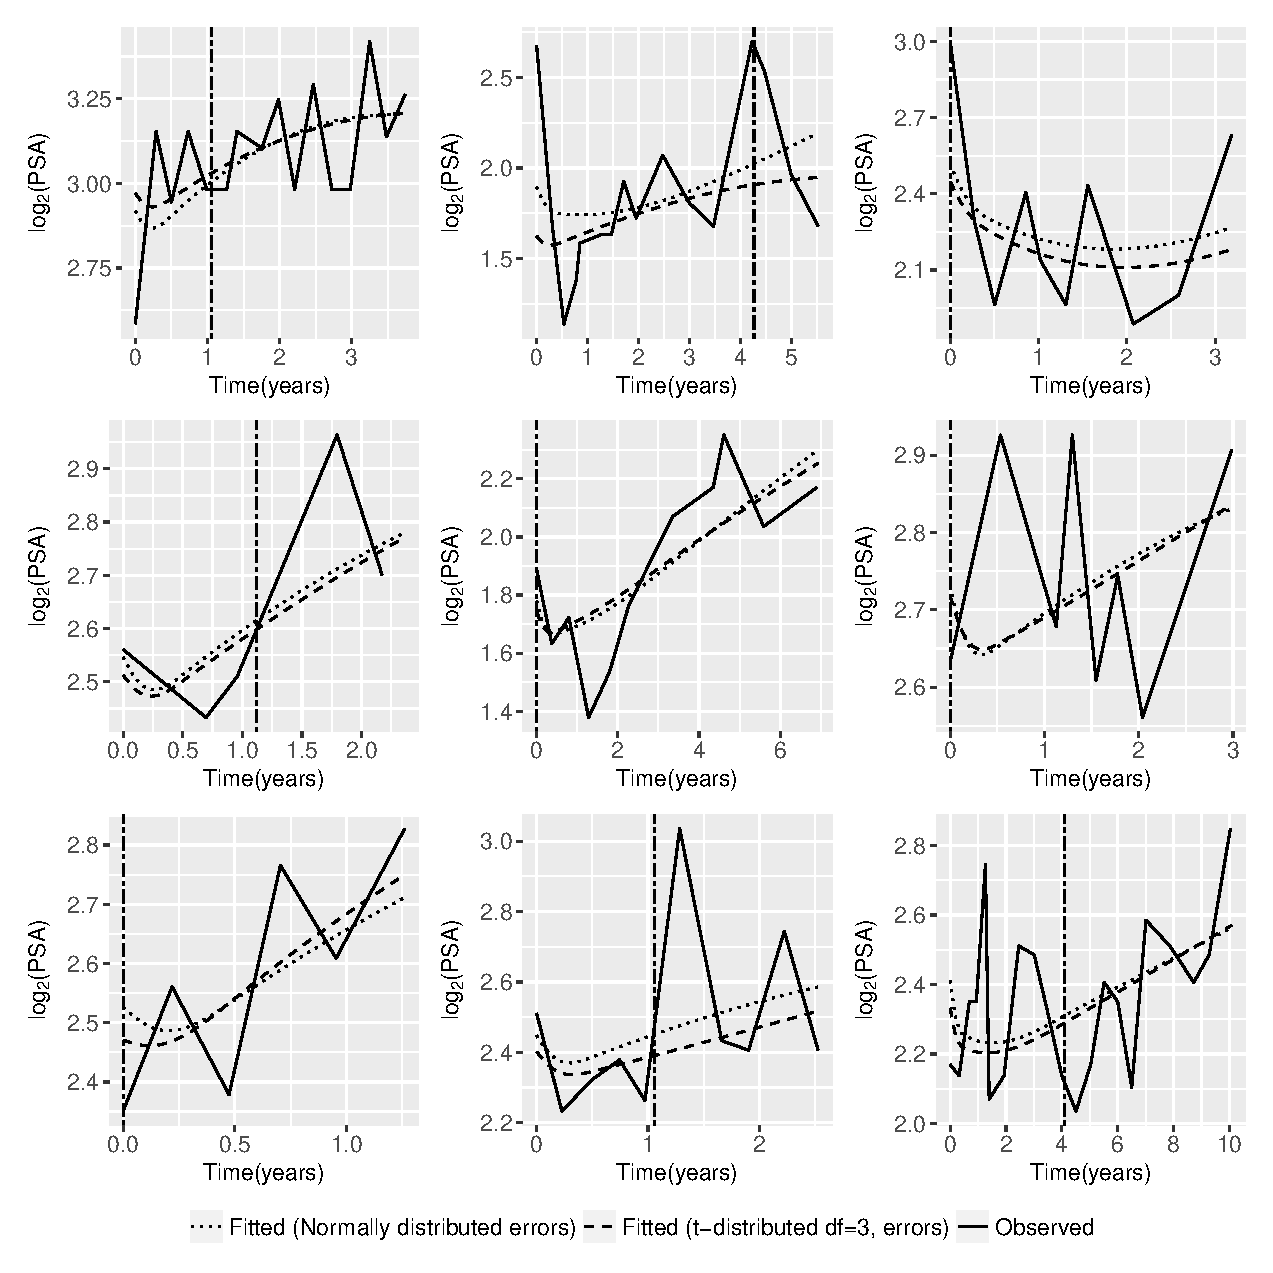
\includegraphics[width=\columnwidth]{images/model_fit/subject_fittedVsObserved_psa_norm_t3.eps}}
    \caption{Fitted versus observed $\log_2 \mbox{PSA}$ profiles for 9 randomly selected patients. Fits were obtained from joint models with assumption of normal distributed errors, and t-distributed (df=3) errors. The fitted profiles utilize information from both the observed PSA levels and time of latest biopsy.}
    \label{fig : subject_fittedVsObserved_psa_norm_t3_ref2}
    \end{figure}

    With regards to the fitted profiles for the three demonstration patients, we show their fitted profiles in Figure \ref{fig : fitted_demo_patients_norm_t3}. The fitted profiles are dynamic in nature, and utilize information from both the observed PSA levels and time of latest biopsy. The first two panels for each of the patients are corresponding to the time points at which we made personalized schedules for these patients in the original manuscript. The third panel for each patient shows the fitted profile for the entire follow up period.

    We have added the aforementioned figures in Web Appendix C of the revised supplementary material as well.
    
    \begin{figure}[!htb]
	\centerline{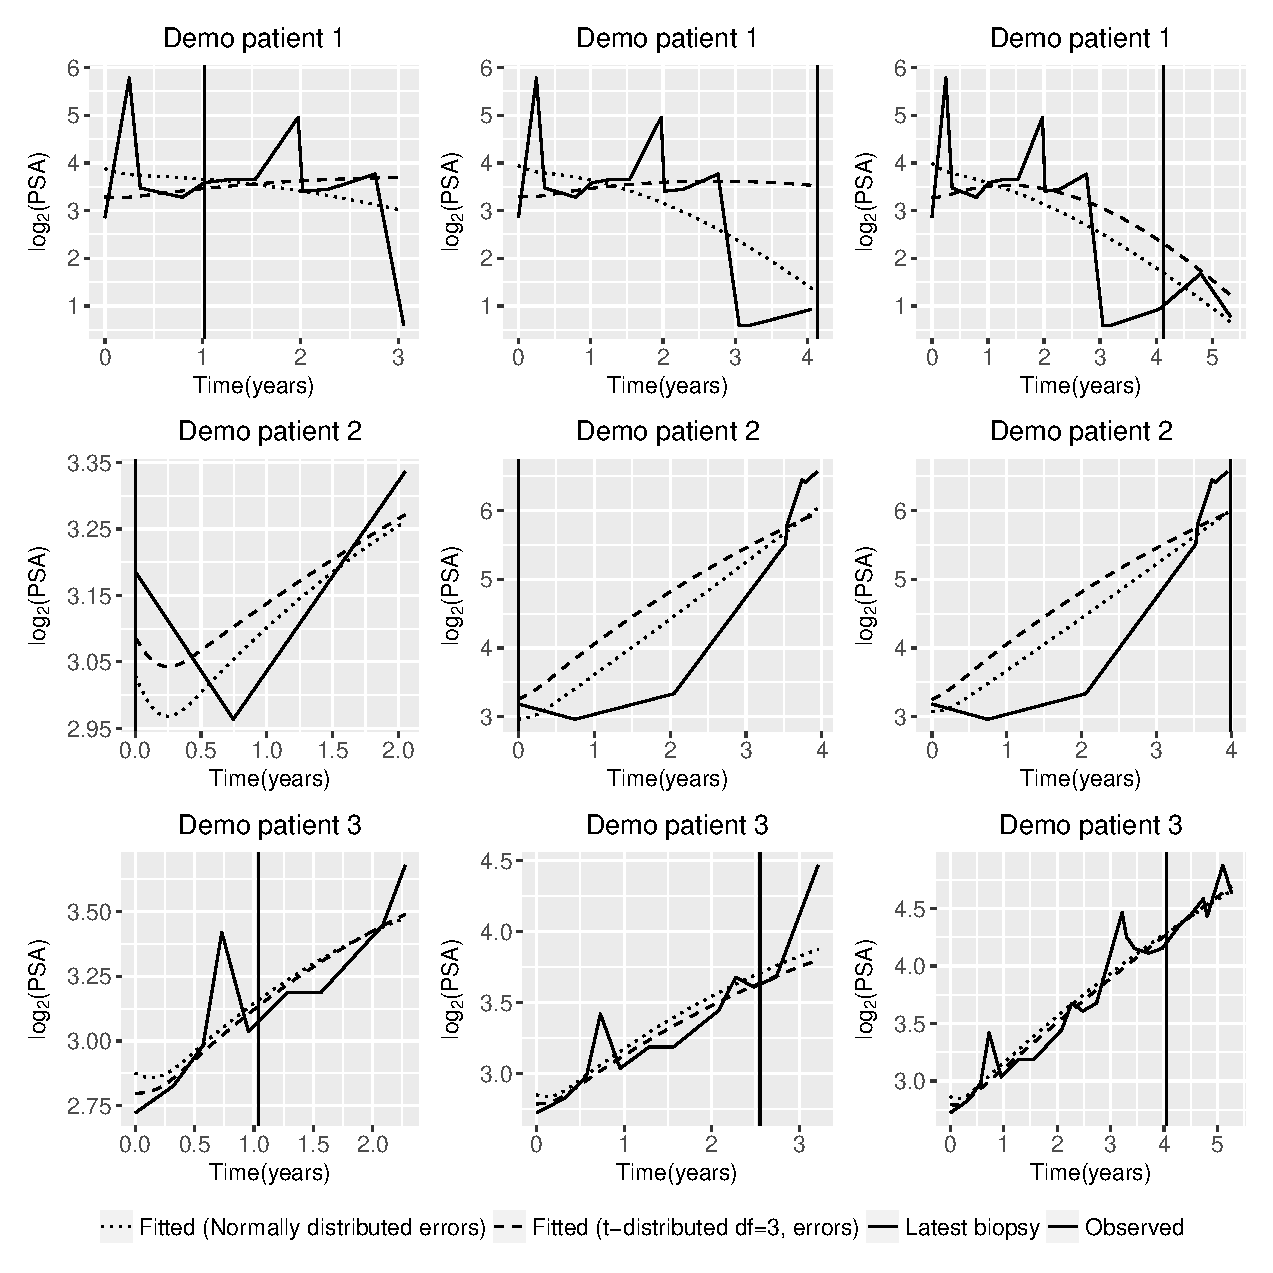
\includegraphics[width=\columnwidth]{images/model_fit/fitted_demo_patients_norm_t3.eps}}
	\caption{Fitted versus observed $\log_2 \mbox{PSA}$ profiles for the three demonstration patients, at two different time points. The fitted profiles are dynamic in nature, and utilize information from both the observed PSA levels and time of latest biopsy.}
	\label{fig : fitted_demo_patients_norm_t3}
	\end{figure}

    \item[2.] \underline{If expected $T^*_j$ is in past, we should be able to suggest to take biopsy right now.}

    We agree to the Reviewer that our approach should be dynamic, that is, it should be able to take into account entire PSA history and repeat biopsies, and also give a decision on immediate/delayed biopsy. We indeed provide a method to \say{evaluate biopsy time from current time, particularly when there is new information, such as new PSA measure after last biopsy}. To illustrate this, suppose for the $j$-th patient, the last biopsy was conducted at time $t$, and the current visit time at which PSA is measured is $s > t$, then we are interested in finding the time $u > s$ of the next biopsy which utilizes all the available information up to $s$. To this end, all of our approaches are based on the posterior predictive distribution of GR time, given by $p\big\{T^*_j \mid T^*_j > t, \mathcal{Y}_j(s), \mathcal{D}_n\big\}$. Here $\mathcal{Y}_j(s)$ is the history of PSA up to $s$ and the information that no GR was found at last biopsy is included via the condition $T^*_j > t$. Indeed as the referee noted it is possible that $t <T^*_j \leq s$, and then biopsy should be conducted immediately. However, it is often the case that difference between consecutive biopsies is required to be at least an year. Thus even if the schedule also suggests a time $t < u \leq s$, the biopsy should not be conducted immediately, but rather with a delay of $1 - t$. We explain this scenario in Section \ref{subsec : pers_sched_algorithm} of the original manuscript. In addition, we have shown the entire decision making process related to conducting a biopsy in the flowchart in Figure \ref{fig : sched_algorithm_ref2} (it is Figure \ref{fig : sched_algorithm} of the original manuscript).

    \begin{figure}
\centerline{\resizebox{0.65\columnwidth}{!}{%

\begin{tikzpicture}
\node (start) [startstop] {
Enter Active Surveillance.
\begin{enumerate}
\item Conduct a biopsy.
\item Set $t=T^{nv}=0$ 
\item Set $u = \infty$
\end{enumerate}
};

\node (takePSA) [process_wide_5cm, below=1cm of start] {
\begin{enumerate}
\item Measure PSA at $T^{nv}$ 
\item Set $s=T^{nv}$
\end{enumerate}
};

\node (propTime) [process_wide_3pt5cm, below=1cm of takePSA] {
\begin{enumerate}
\item Set $u^{pv} = u$ 
\item Update $g(T^*_j)$ 
\item Propose $u$
\end{enumerate}
};

\node (decision1) [decision, below = 1.5cm of propTime] {$u < u^{pv}$};
\node (pro6) [process, right = 1.35cm of decision1] {Set $u = u^{pv}$};

\node (decision5) [decision, left=1.5cm of decision1] {$u \leq s$};

\node (pro5) [process, below=1.5cm of decision5] {Set $u = s$};

\node (decision2) [decision, below=0.5cm of decision1] {$u - t > 1$};

\node (decision4) [decision, right=1.5cm of decision2] {$u > T^{nv}$};

\node (pro3) [process_wide_3pt5cm, below=1cm of decision2] {
\begin{enumerate}
\item Conduct Biopsy at $t + 1$ 
\item Set $t = t + 1$
\end{enumerate}
};

\node (pro4) [process_wide_3pt5cm, below=1cm of decision4] {
\begin{enumerate}
\item Conduct Biopsy at $u$
\item Set $t = u$
\end{enumerate}
};

\node (decision3) [decision, below=1cm of pro3] {$\mbox{Gleason} > 6$};
\node (pro7) [process, left=1cm of decision3] {Set $u=\infty$};

\node (stop) [startstop, below = 1cm of decision3] {Remove patient from AS};

\draw [arrow] (start) -- (takePSA);
\draw [arrow] (takePSA) -- (propTime);
\draw [arrow] (propTime) -- (decision1);
\draw [arrow] (decision1) -- node[anchor=south] {Yes} (decision5);
\draw [arrow] (decision5) -- node[anchor=east] {Yes} (pro5);
\draw [arrow] (pro5) -- (decision2);
\draw [arrow] (decision1) -- node[anchor=south] {No} (pro6);
\draw [arrow] (decision5) -- node[anchor=south] {No} (decision2);
\draw [arrow] (pro6) -- (decision4);
\draw [arrow] (decision4.east) |- ([xshift=0.35cm, yshift=-4.15cm]pro6.north east) |- node[anchor=south] {Yes} (takePSA);
\draw [arrow] (decision2) -- node[anchor=south] {Yes} (decision4);
\draw [arrow] (decision2) -- node[anchor=east] {No} (pro3);
\draw [arrow] (pro3) -- (decision3);
\draw [arrow] (pro4) |- (decision3);
\draw [arrow] (decision3) -- node[anchor=east] {Yes} (stop);
\draw [arrow] (decision4) -- node[anchor=east] {No} (pro4);
\draw [arrow] (decision3) -- node[anchor=south]{No} (pro7);
\draw [arrow] (pro7.west)|- ([xshift=-0.35cm, yshift=-7.8cm]pro5.north west) |- (propTime);
\end{tikzpicture}

}%

}
\caption{Algorithm for creating a personalized schedule for patient $j$. The time of the latest biopsy is denoted by $t$. The time of the latest available PSA measurement is denoted by $s$. The proposed personalized time of biopsy is denoted by $u$.  The time at which a repeat biopsy was proposed on the last visit to the hospital is denoted by $u^{pv}$. The time of the next visit for the measurement of PSA is denoted by $s^{nv}$.} 
\label{fig : sched_algorithm_ref2}
\end{figure}

    We would also like to take the opportunity and provide extra clarification for the definition of $\mathcal{M}_i(t)$ on page 5 of the original manuscript. We define $\mathcal{M}_i(t) = \{m_i(v), 0\leq v \leq t\}$ as the history of the underlying PSA levels up to time $t$, or as noted by the Referee, PSA level up to last biopsy \citep{tsiatis2004joint,rizopoulos2012joint}. The reason for such a definition is that the association between hazard of GR and PSA may depend on the entire history of PSA levels. For example, if hazard of GR at time $t$ depends on the cumulative PSA levels up to $t$, then it is manifested by the following functional form:
    
    \begin{equation}
    f\{\mathcal{M}_i(t), \boldsymbol{b}_i, \boldsymbol{\alpha}\} = \alpha \int_0^t m_i(t) \rmn{d}{t}
    \end{equation}

    \item[3.] \underline{Robustness of the schedules based on dynamic risk of GR}
    
    We agree with the Referee that the term robust was used inappropriately. The meaning we wanted to imply was that schedules based on dynamic risk of GR are robust to large overshooting margins (offset). We observed in Figure \ref{fig : prias_demo_pid_911} of the original manuscript that the variance of posterior predictive distribution of event time decreases as more information is gathered over time. That is, a schedule based on expected/median time of Gleason reclassification (GR) is less accurate (the consistency property) in predicting true event time when less information is available. In comparison, the schedule based on dynamic risk of GR is robust in the sense that it is more risk averse than the schedule based on median time of GR (50\% risk), at all time points. For example, in PRIAS, on average it schedules biopsies whenever the risk increases more than 5.3\%. Thus, it is less likely to overshoot the true GR time by a big margin even if less information is available for the patients. This is also demonstrated via the simulation study, wherein the schedule based on dynamic risk of GR leads to almost the same mean offset and variance of offset across the three subgroups of patients. 

    Due to space restrictions in the main manuscript we have provided the following brief explanation. In practice, for some patients we may not have sufficient information to accurately estimate their PSA profile. The resulting high variance of $g(T^*_j)$ could lead to a mean (or median) time of GR which overshoots the true $T_j^*$ by a big margin. In such cases, the approach based on dynamic risk of GR with smaller risk thresholds is more risk averse and thus could be more robust to large overshooting margins. 

\end{enumerate}

\subsection*{Minor Concerns Shared by the 2nd Referee}

\begin{enumerate}
	\item[1.] \underline{More informative captions for tables and graphs.}

    We have now updated the captions of tables and graphs in the revised version of the manuscript. We specifically mention that these graphs pertain to the results from the simulation study.
	
    \item[2.] \underline{Recommended values for parameters $\kappa$ and $\eta$.}

    For the two parameters $\kappa$ and $\eta$, we do not use fixed set of values. We compute the parameter $\kappa$ (dynamic risk of GR) from the data, as shown in Section \ref{subsec : estimation} of the original manuscript. That is, we obviate choosing this value manually. We also provide an example for a commonly recommended risk threshold of 5\%. It is quite a risk averse threshold, however as shown in \ref{table : sim_study_pooled_estimates_extended} in supplementary material the performance of this schedule is exactly same as that of annual schedule. That is, it gives a very small offset at the cost of too many biopsies.

	With regards to the choice of weights $\eta_1, \eta_2$, as discussed in Section \ref{subsec : optimal_schedule} of the original manuscript, this choice can be obviated by reformulating the optimization of original weighted sum as a constrained optimization problem. For example, if $\eta_1$ is the weight corresponding to average number of biopsies $E(N^S)$ and $\eta_2$ is the weight corresponding to average offset $E(O^S)$, then we can instead put a constraint $C$ on average offset, and then optimize for only the number of biopsies. The choice of offset cutoff $C$ is discussed in point number 4 below.

	\item[3.] \underline{Age effect is not interpretable because of quadratic form of age.}

    We thank the Referee for noticing that due to the quadratic form of age in our model, the interpretation of relative difference of age that we did is incorrect. We have addressed this issue in our revised manuscript. We now illustrate the effect of age with an example, namely an increase in age at the time of inclusion in AS from 65 years to 75 years (first and third quartiles of age in PRIAS dataset) corresponds to a 1.419 fold increase in the hazard of GR.

 \item[4.] \underline{Good and bad $O^S_j$ and $N^S_j$}

 The Reviewer raises a very important point with regards to the practicality of our approach. In this regard, the discussion of good and bad $O^S_j$ and $N^S_j$ entails discussion of patients tolerance for burden ($N^S_j$), and the amount of risk($O^S_j$) that doctors consider manageable. Hence there are no fixed cutoffs for good and bad $O^S_j$ and $N^S_j$. However, because PRIAS and annual schedules are already in practice, it can be argued that the maximum possible offsets due to these schedules (one and three years, respectively) are acceptable to doctors. In addition, multiple studies have reported small PCa specific mortality in low risk AS patients \citep{loeb2016immediate,tosoian2011active,klotz2009clinical}. Thus, less frequent schedules are an interesting alternative. For example, for slowly progressing patients in our simulation study, we observed that the schedule based on expected time of GR conducts on average two biopsies and has an average offset of 10 months. In comparison, annual schedule conducts six biopsies on average and gives an offset smaller by only four months, making the personalized schedule a suitable alternative. 

 For high risk patients however, early detection (annual or PRIAS schedule) may be necessary, given the rapidness of progression. When it is not known in advance if a patient will have a fast or slow progression of PCa, the hybrid approach may be used. It conducts one biopsy less than the annual schedule in faster progressing PCa patients and has an average offset of 10.25 months. For slowly progressing PCa patients it conducts two biopsies less than the annual schedule and has an average offset of 8.55 months.

\end{enumerate}

